% PART 5: Practical Implementation
\chapter{Practical Implementation}
The Project repositories are hosted on GitHub, are public and can be accessed by following these references: Back-end Core Logic\cite{alexei_pavlovschii_blocksign_nodate} and Front-end User Interface\cite{vladimir_vitcovschii_blocksign_nodate}.

\section{Back-end architecture}
The back-end of the system has been developed with a focus on scalability, modularity, and security. Its purpose is to provide all the critical functionality required for user registration, authentication, document management, and secure verification of signatures (Figure \ref{main-project-routers}). 

\begin{figure}[H]
    \centering
    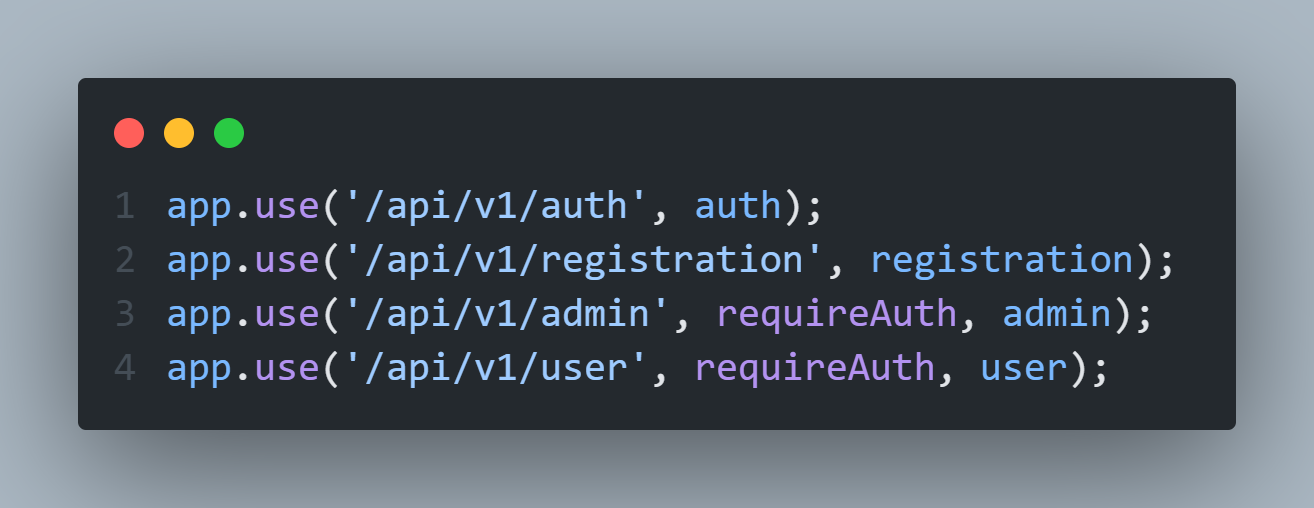
\includegraphics[width=18cm]{"images/main-project-routers.png"}
    \caption{Main Project Routers}
    \label{main-project-routers}
\end{figure}

The implementation relies on Node.js with the Express.js framework, while data persistence is handled by PostgreSQL through the Prisma ORM.

\subsection{Application Layer}
The server is structured around separate route modules, each of which is responsible for a specific part of the functionality. For example, the auth.routes.ts file manages the passwordless login process using challenge–response verification, while registration.routes.ts covers the steps of email OTP verification, registration requests, and account completion with a public key. The administrator’s responsibilities, such as reviewing and approving registration requests, are implemented in admin.registration.routes.ts. Finally, user-oriented functionality, including profile management and document operations, is centralized in user.routes.ts. This modular design improves maintainability and makes it easier to extend the system in the future.

\subsection{Database Layer}
The database schema is implemented using Prisma ORM on top of PostgreSQL. Entities such as User, RegistrationRequest, Document, DocumentParticipant and Signature are modeled explicitly with foreign keys and unique constraints to guarantee consistency (Figure \ref{user-db-model}). 

\begin{figure}[H]
    \centering
    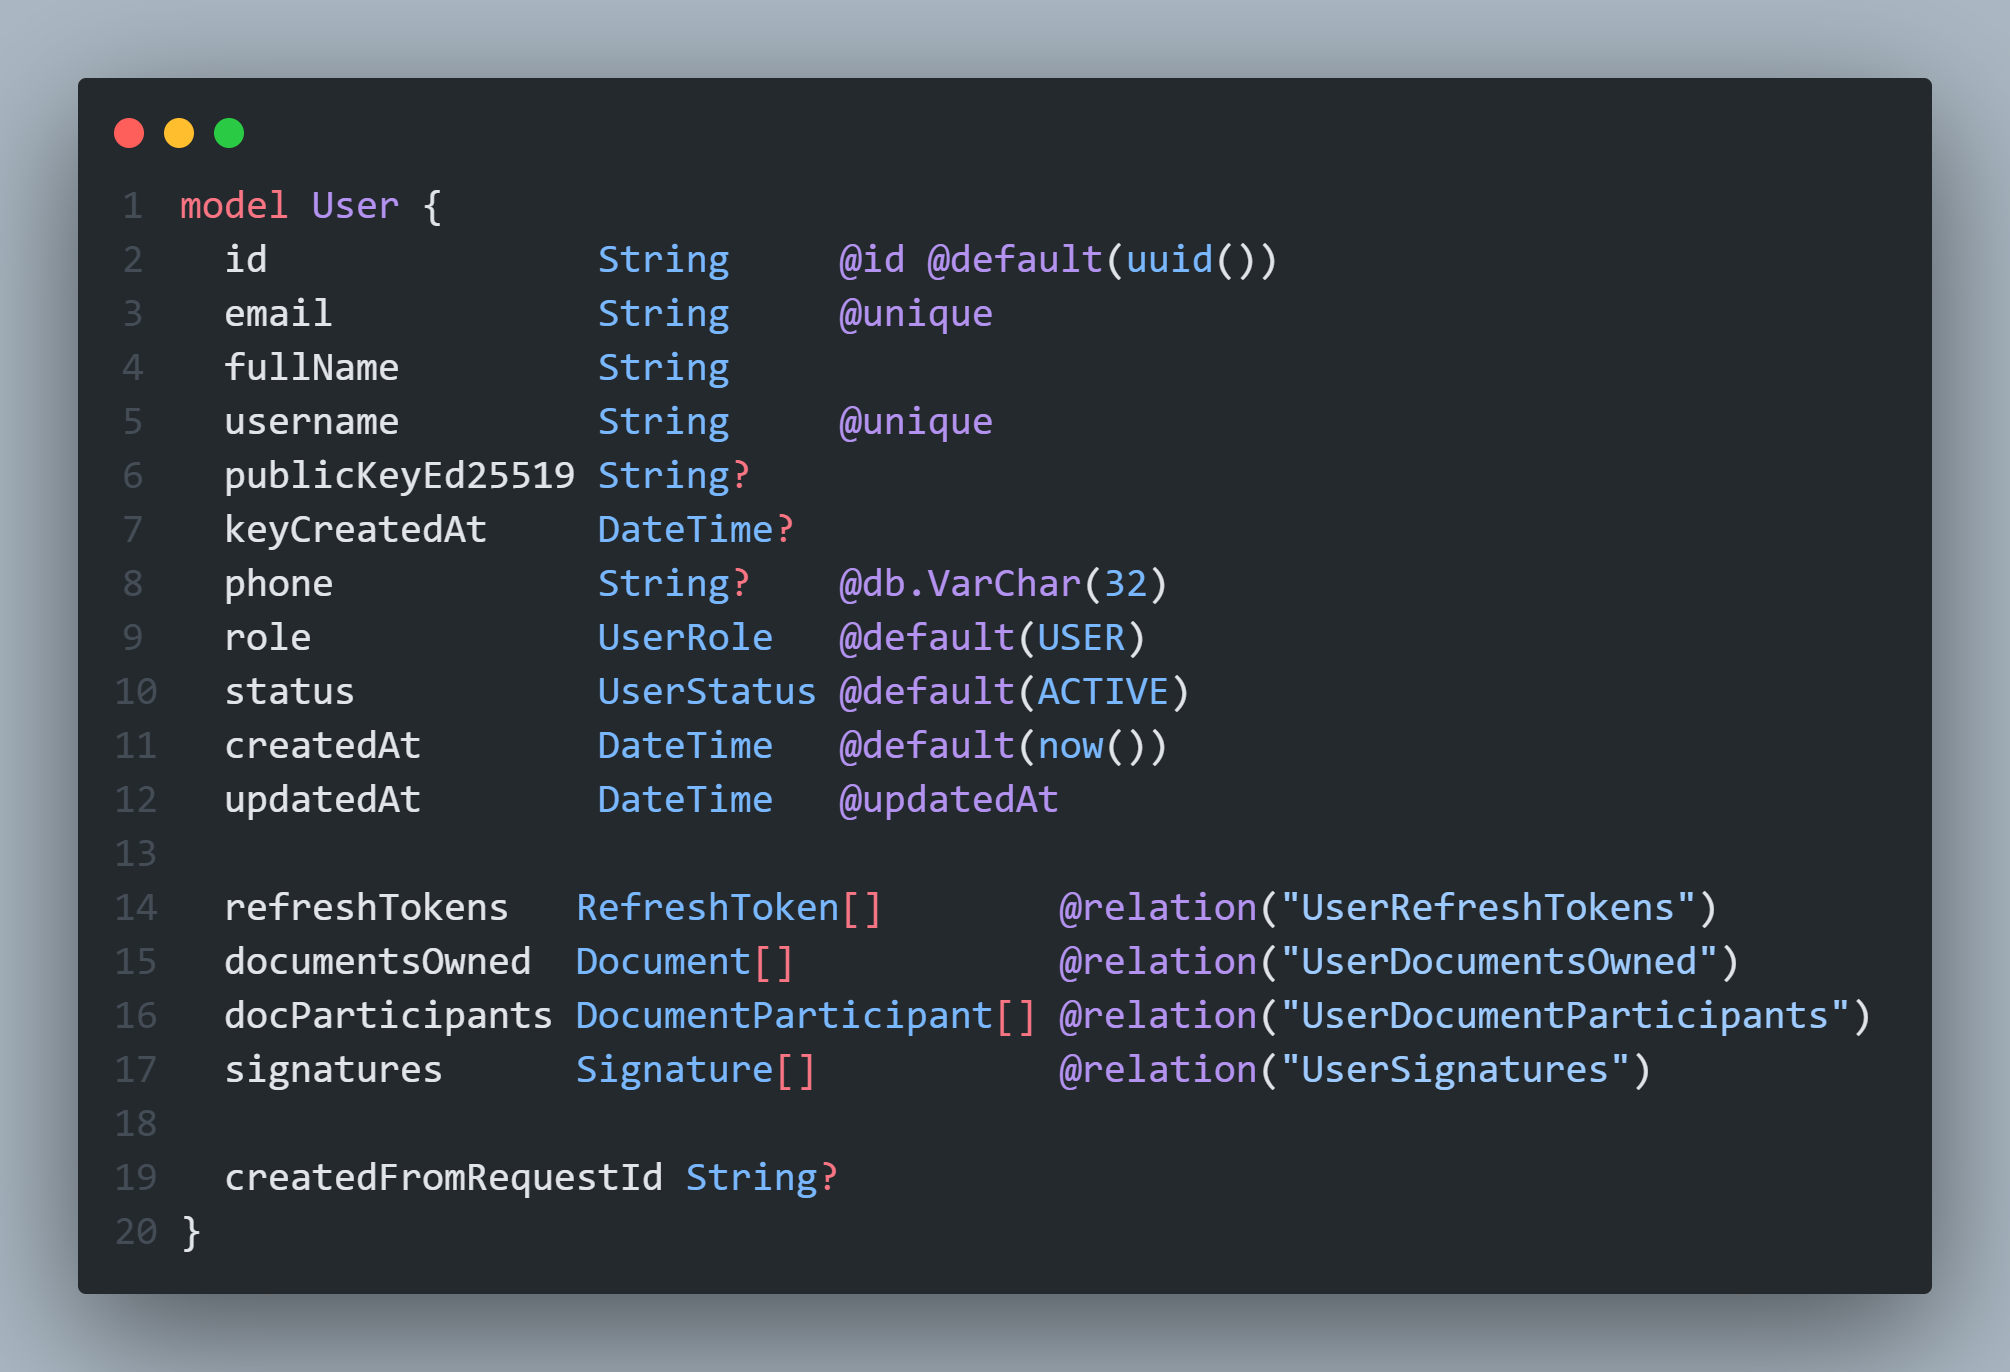
\includegraphics[width=18cm]{"images/user-db-model.png"}
    \caption{User Database Model}
    \label{user-db-model}
\end{figure}

The use of Prisma Client enables type-safe queries and simplifies operations like migrations, seeding, and testing.

\subsection{Security Measures}
The architecture incorporates several security mechanisms. Authentication challenges are valid only for five minutes and become invalid once used. Refresh tokens are stored in secure cookies to reduce exposure. The use of Ed25519 ensures modern cryptographic security, while SHA-256 guarantees the integrity of documents. Finally, file validation ensures that only PDF documents are accepted.

\subsection{Authentication and Tokens}
Authentication in the system is fully passwordless and relies on public/private key pairs. Users prove their identity by signing challenges provided by the server. Successful verification grants them access tokens and refresh tokens in the form of JWTs.

Access tokens are short-lived and returned in the response body, while refresh tokens are long-lived and stored securely in HTTP-only cookies. Middleware functions such as requireUser and requireAdmin check the validity of tokens and enforce role-based access control.

\subsection{Email Service}
The system integrates Nodemailer as an email delivery mechanism configured with SMTP credentials for the project’s domain. Emails are used in two important contexts. First, during registration, users receive a six-digit OTP code for email validation. Second, during document workflows, participants receive notifications when they are asked to review and sign a document, and again when the document has been finalized (Figure \ref{email-sending}).

\begin{figure}[H]
    \centering
    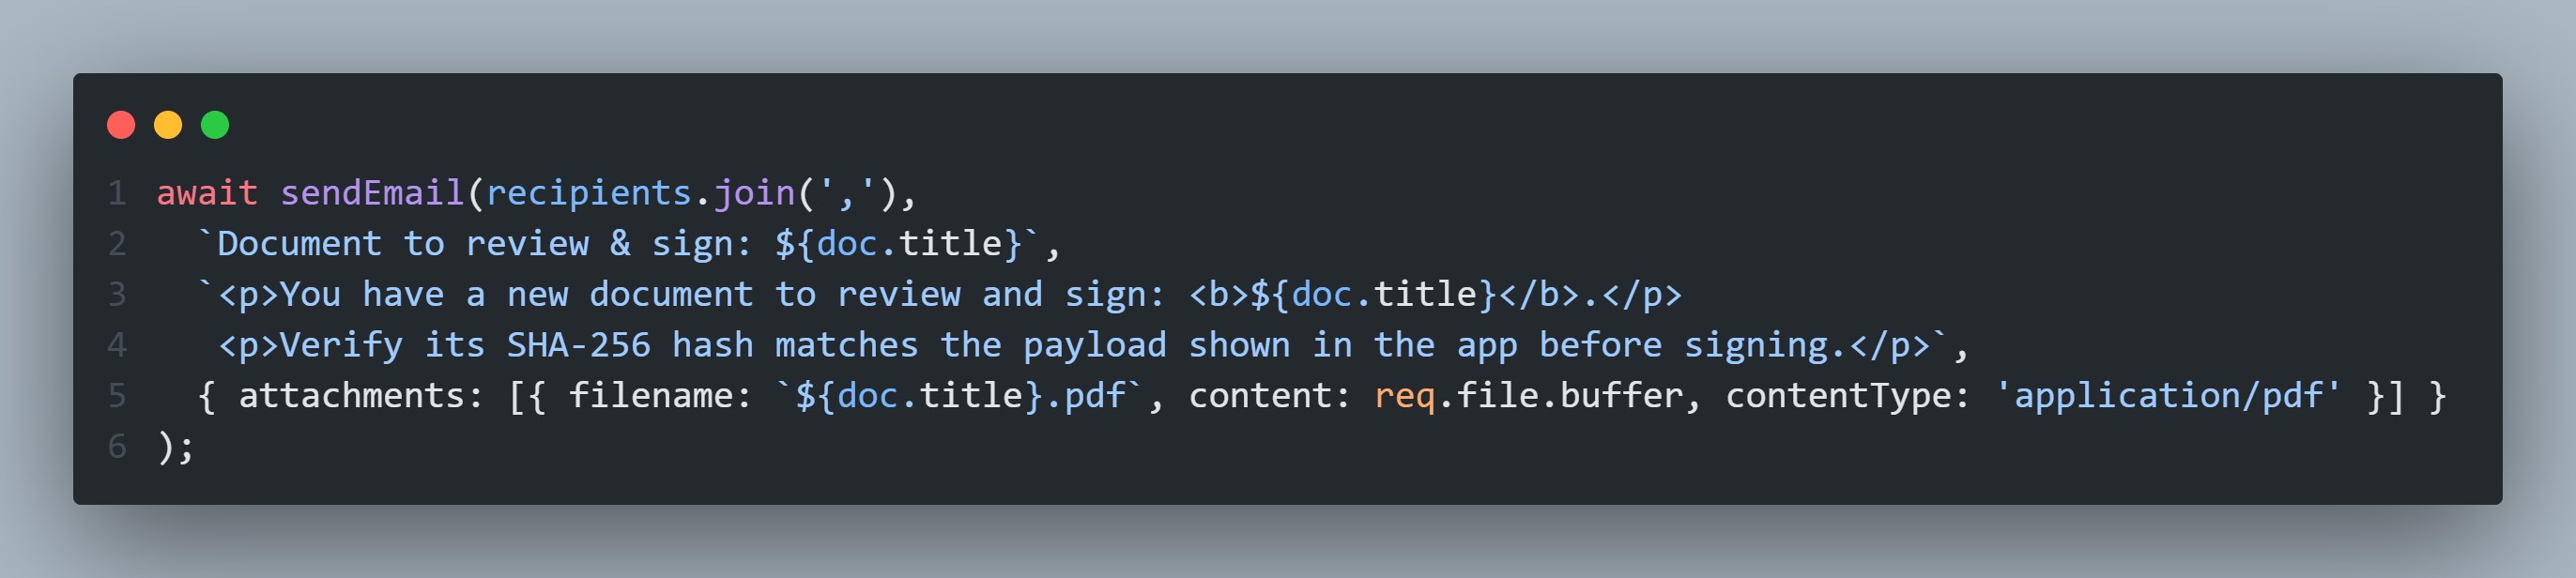
\includegraphics[width=18cm]{"images/email-sending.png"}
    \caption{Email Sending Mechanism}
    \label{email-sending}
\end{figure}

\subsection{Cryptographic Module}
Security of authentication and documents is achieved with the Ed25519 digital signature scheme, implemented via the @noble/ed25519 library (Figure \ref{keygen}). 

\begin{figure}[H]
    \centering
    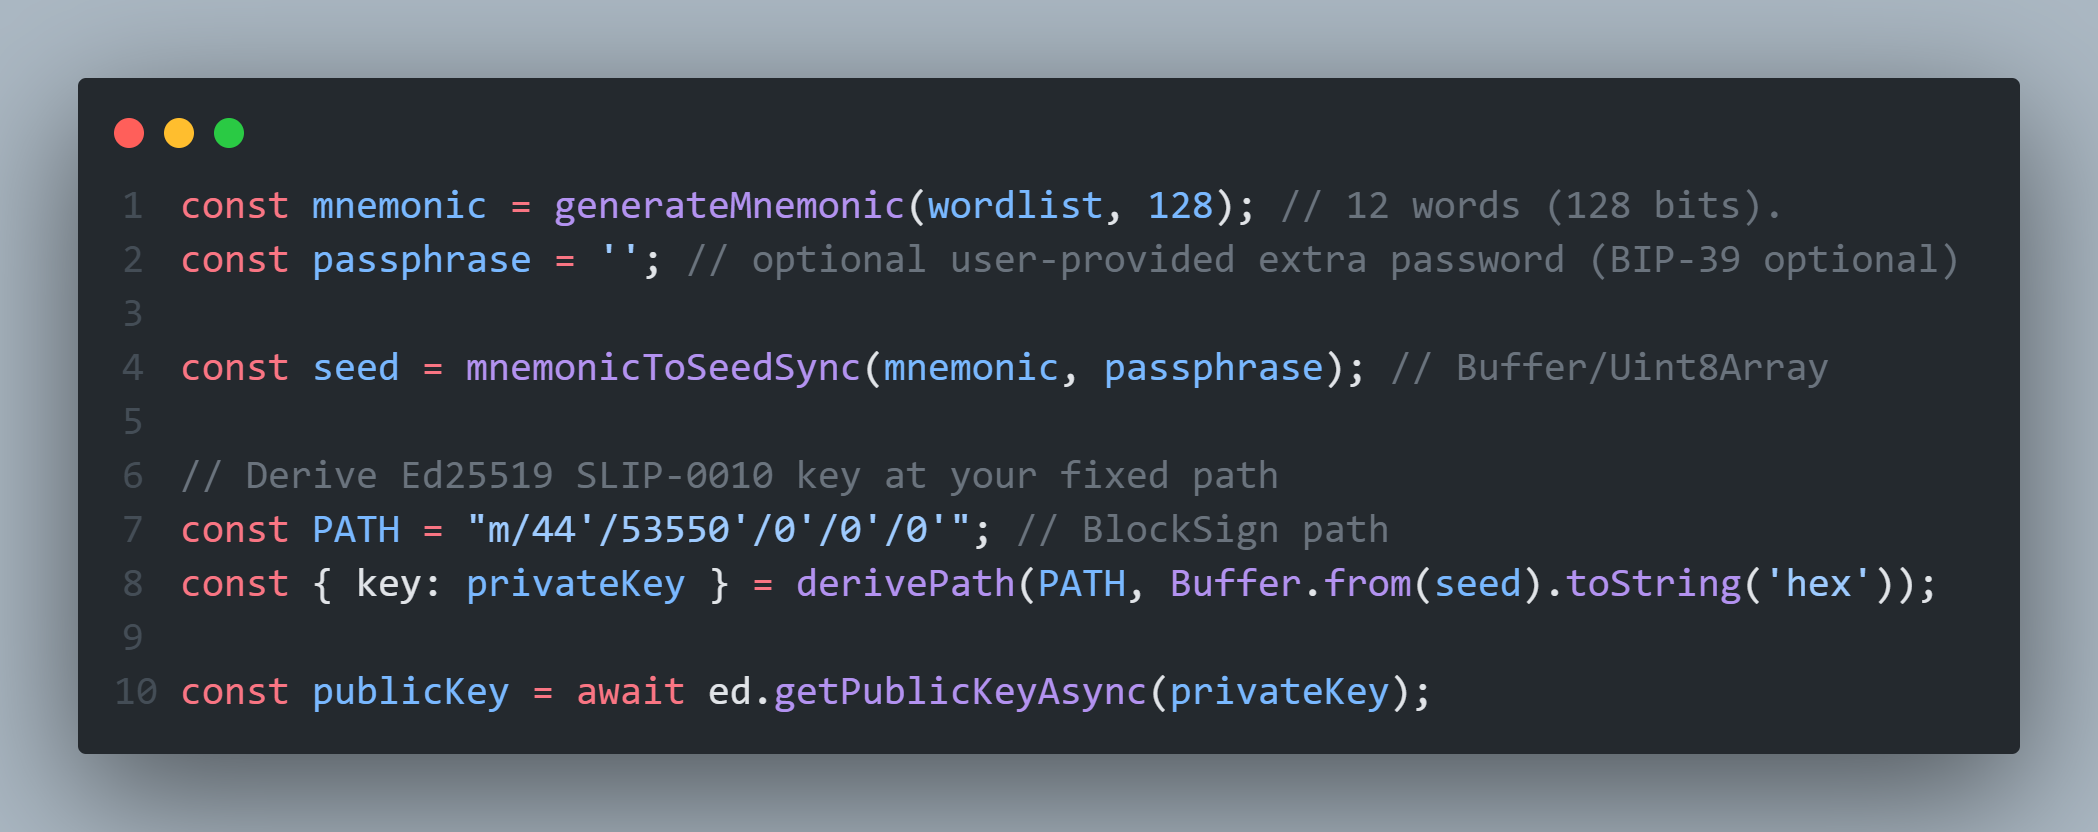
\includegraphics[width=18cm]{"images/keygen.png"}
    \caption{Key Pairs Generation Mechanism}
    \label{keygen}
\end{figure}

A dedicated crypto utility handles key pair generation, signing, and verification of messages. In addition, SHA-256 is used for hashing documents, ensuring their integrity before they are accepted or signed.

\subsection{Document Workflow}
The MVP implementation of the document signing process follows a well-defined lifecycle. When a user creates a document, they upload the file, calculate its SHA-256 hash, and sign a canonical payload. The payload and initial signature are stored in the database.

Participants selected by the creator receive an email with the PDF attached and the corresponding hash. Each participant is expected to calculate the hash independently, compare it with the payload, and if it matches, sign the document (Figure \ref{payload-signature}). 

\begin{figure}[H]
    \centering
    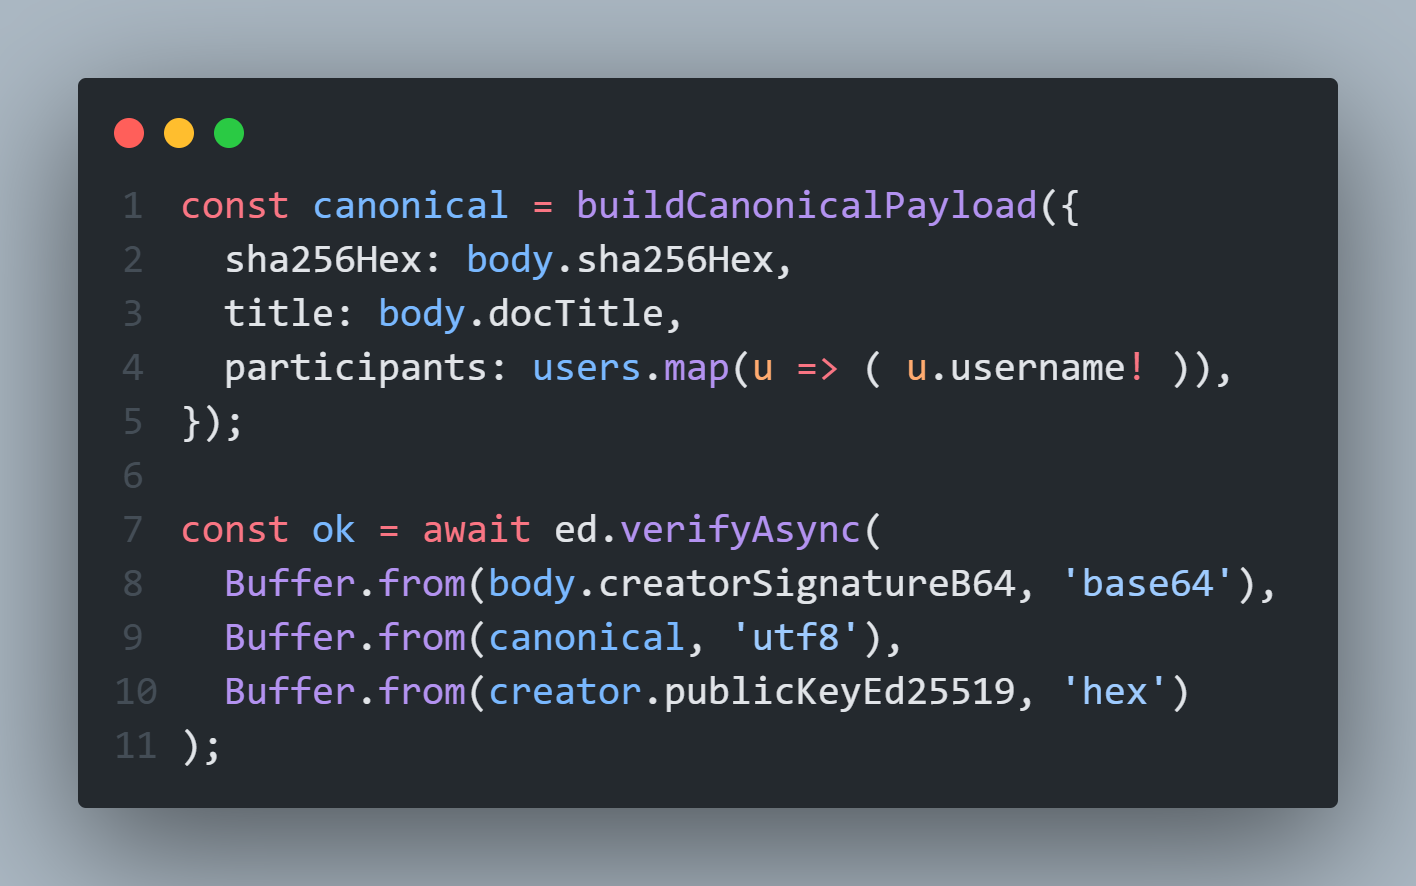
\includegraphics[width=18cm]{"images/payload-signature.png"}
    \caption{Build Paylaod and Verify Signature}
    \label{payload-signature}
\end{figure}

Their signatures are then added to the database. Once all required signatures are collected, the document status changes to signed, and a notification is sent to all involved parties.

\subsection{Extensibility}
The modular design of the back-end makes it adaptable to future improvements. Currently, documents are distributed as email attachments, but the system is ready for integration with external storage providers such as AWS S3. The ChainAnchor entity in the future versions of database will anticipate the anchoring of finalized document hashes on blockchain networks. Similarly, while usernames are currently used to tag participants, the design leaves room for later integration with decentralized identity systems.

\section{Front-end UI}
Aa
